\section{\textbf{The FSMDriver}} \label{sec:FSM}
	
	Some of the main aspects discussed to outline a controller for TORCS were sufficed by the concept of Finite State Machines (FSM)~\cite{Millington:2006:FSM}, the most important one being the goal of reaching autonomous driving behavior in a car race.

	According to Mat Buckland in \emph{Programming Game AI By Example}~\cite{Buckland:2005:AI}:
	
	\begin{quotation} \itshape
		
		``A finite state machine is a device, or a model of a device, which has a finite number of states it can be in at any given time and can operate on input to either make transitions from one state to another or to cause an output or action to take place. A finite state machine can only be in one state at any moment in time.''
		
	\end{quotation}
	
	This architecture was chosen in order to transform the problem of complex driving into smaller problems that describe the situations found within the racing environment.
	
\subsection{The Design of the Behavior States}
	
	Initially, the design of the finite-state machine proposed comprised the following states:
	
	\begin{itemize}

	\item \emph{Straight Line};
	
	\item \emph{Approaching Curve};
	
	\item \emph{Curve};
	
	\item \emph{Out of Track};
	
	\item \emph{Stuck}.

	\end{itemize}
	
	Essentially, for the first method, normal behavior covered \emph{Straight Line}, \emph{Approaching Curve} and \emph{Curve}, as the controller was located inside the track boundaries and no recovery actions needed to be considered, whereas exception behavior consisted of \emph{Out of Track} and \emph{Stuck}, situations in which such conduct was expected.
	
	The main difference between the method described and the second one is the way they deal with normal behavior, while one separates it into \emph{Straight Line}, \emph{Approaching Curve} and \emph{Curve}, the other treats it as a unique conduct in the form of the \emph{Inside Track} state. Therefore, the modified finite-state machine was composed by only three states, which were:
	
	\begin{itemize}
		
		\item \emph{Inside Track};
		
		\item \emph{Out of Track};
		
		\item \emph{Stuck}.
		
	\end{itemize}
	
\subsubsection{Normal Behavior}
	
	If a controller using the first method was currently in \emph{Straight Line}, it would be expected of him to simply go as fast as he could, with no steering changes whatsoever. When in \emph{Approaching Curve} state, he would reposition himself proportionally to the curvature of the approaching curve in order to achieve higher speeds once inside it. For example, if there is a sharp left turn nearby, the controller sets a target steer that the car needs to obtain before entering it, while bringing the car further to the right of the lane; that way, when the left turn comes, the car can proceed with a less abrupt change of steer, which results in a higher speed. Otherwise, when in situations of \emph{Curve}, the pilot would stop braking while maintaining the steering direction towards the sensor pointing the biggest distance value read - which represents the direction of the curve, prepared by the approaching curve state. Figure~\ref{Fig:FSensor} exhibits a car receiving information from the sensors, with the biggest vector being the direction of the curve to be entered.
	
	\begin{figure}[h]
		
		\centering
		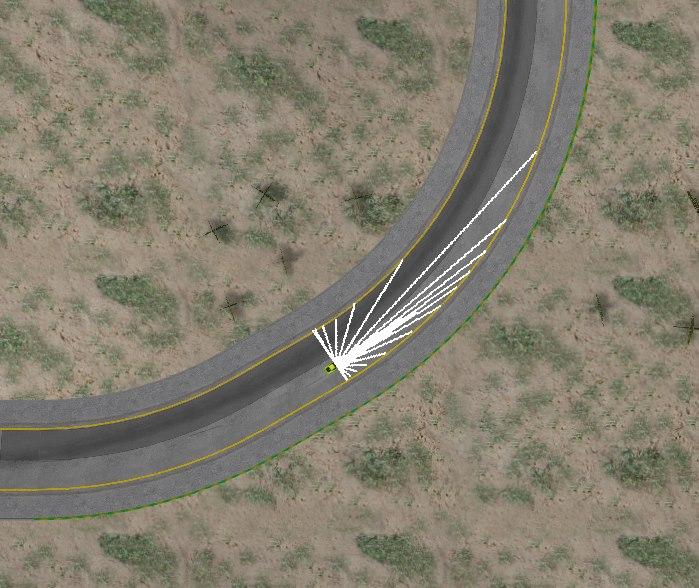
\includegraphics[width=250pt]{FarthestSensor}
		\caption{Sensorial input indicating a curve through the biggest value received}
		\label{Fig:FSensor}
		
	\end{figure}
	
	\emph{Inside Track}, therefore, is how the car, desirably, will spend most part of the time, if the second method is being employed. The controller calculates a \emph{target speed} based on how far the car is from the farthest edge of the track, then, it assumes a position of increasing the speed until it reaches this velocity while driving towards the sensor with the biggest read value. The distance of this method conveys the greater length the car may advance with little or sometimes without significant steer changes. This state also brakes, if necessary, in situations that the car assumes a speed higher than the one calculated to be the target.
	
\subsubsection{Exception Behavior}
	
	For the exception states, even though the expected deportment is well known, e.g. a stuck controller should maneuver the car out of the current situation and proceed to normal race conduct, the implementations vary among developers. The policies chosen for the exception states were used on both proposals equally as a matter of regularity of comparison.
	
	\emph{Out of Track} is when, for any unknown reason, the car is found outside of the track limits. In this case, the proper behavior is to try to return to the lane. In road tracks, the outside track normally has a different terrain, sometimes dirt-based, meaning that skidding frequently occurs, and in an effort to avoid this, a control system to brake when the car begins skidding above a threshold was implemented. Since there are many ways that a car may be out of the track, reentering it in an efficient way might require many different angles as well, so, every time the car exceeds the inside boundaries of the lane, a proper returning angle is calculated. \insertPicture{Out of Track desired return angle}.
	
	\emph{Stuck} represents any given situation that the car is unable to progress in the race. This is a delicate state, because it presents itself as difficult to identify and also due to its impact to the performance of the controller. In order to detect \emph{Stuck} circumstances, the speed of the car is monitored throughout the race, during every game tick, if it lingers with a low speed for a determined period, then it is considered stranded, or stuck. When detected, this state activates the reverse gear of the car and turns it until its front is directed towards the correct axis of the track. The reason why \emph{Stuck} is a sensitive state is because, when detected early, might indicate false positive, and, when detected late, could lessen the efficiency of the controller. Thusly, detecting \textit{Stuck} situations is crucial, and so is handling the car out of them.
	
\subsection{Five-State FSM} \label{subsec:FSM5}

	The first method was named ``Five-State FSM'', naturally because it is a finite state machine with five states. The real first model of the finite-state machine did not have an \emph{Approaching Curve} state, but, as the demeanour of \emph{Straight Line} and \emph{Curve} were so different from one another, a preparation had to be established so as to smoothen the transitions between them. Figure~\ref{Fig:FSM5Diagram} represents the states diagram of the Five-State FSM.
	
	\begin{figure}[h]
		
		\centering
		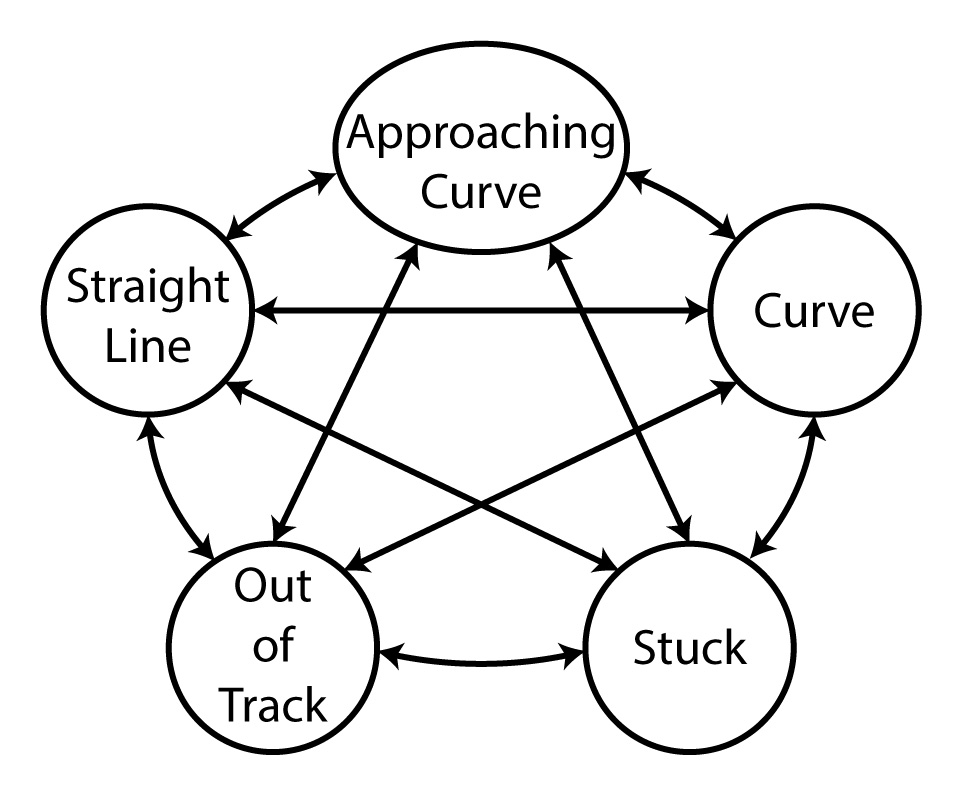
\includegraphics[width=250pt]{FiveStateFSM}
		\caption{States diagram of the Five-State FSM}
		\label{Fig:FSM5Diagram}
		
	\end{figure}
	
	Figure~\ref{Fig:FSM5Diagram} instantiates the relations between the states and the transition function through two-headed arrows, which is done because the function chooses which state the controller is supposed to be, but the states also communicate with it through the actuators that determine indirectly which will be the next state. This way, the states provide a type of feedback.
	
	One big problem about this approach is that the function responsible for choosing which state is more appropriate for each situation would more than often be overcharged, and, in some cases, rather different sets of parameters received by it would result in the same classification among the states. Thus, in order to minimize the dependency of the driving performance in relation to the function in charge of the transition between states, a project decision was made to reduce the number of states.
	
	In addition, the angles - with relation to the car axis - of all the 19 range finder sensor have to be initialized in a manner that includes as much information of the track as possible. For instance, if all the angles were to be initialized pointing only to one side of car, the data concerning the other side would be neglected. For the Three-State FSM, the angles were instantiated using steps of 10 degrees, which results in angles ranging from -90 to +90 degrees - 0 meaning the direction that indicates the front of the car.
		
\subsection{Three-State FSM} \label{subsec:FSM3}
	
	The finite state machine with less states was designed from a derivation of the previous one, by adapting the normal behavior and simplifying it to form the Three-State FSM. The exception behavior remained the same, since it should not affect the car as much if the adaptation was well performed. Figure~\ref{Fig:FSM3Diagram} shows the modified states diagram of the Three-State FSM.
	
	\begin{figure}[h]
		
		\centering
		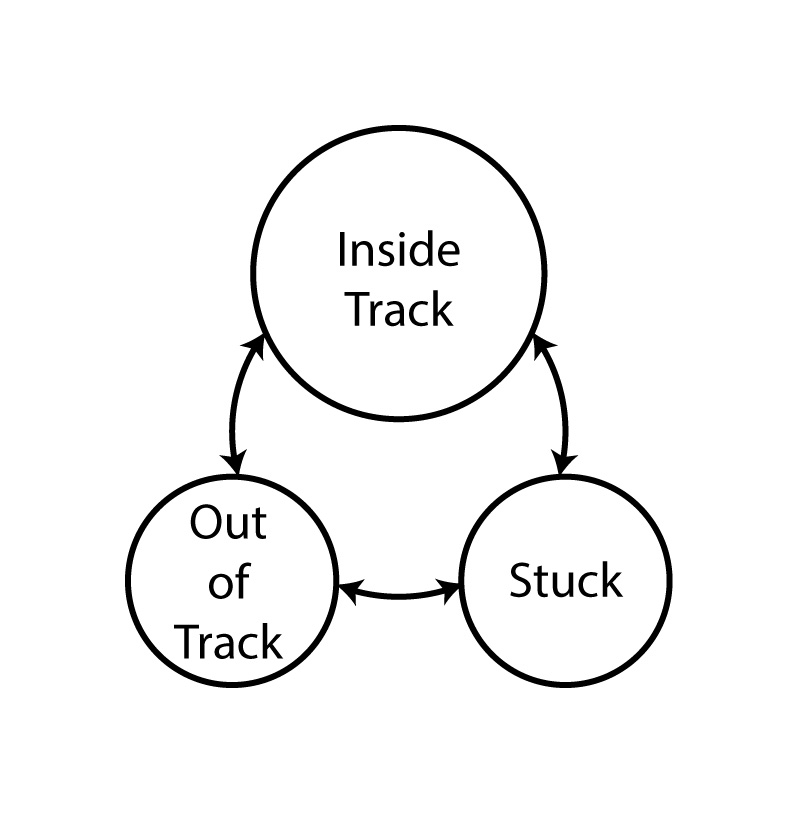
\includegraphics[width=230pt]{ThreeStateFSM}
		\caption{States diagram of the Three-State FSM}
		\label{Fig:FSM3Diagram}
		
	\end{figure}
	
	Even though the Three-State FSM also has a transition function, it does not receive the heavy burden of decision present in the other approach. It mainly checks if the car is \emph{Stuck}, if so, it manages this situation, if not, it checks if the car is \emph{Out of Track} and deals with it as well. Otherwise, the car will be at the \emph{Inside Track} state, which represents most of the racing time - justifying it being bigger in Figure~\ref{Fig:FSM3Diagram}, and also most of the work required from the controller to handle the driving behavior.
	
	Besides the states, there is also a learning module that is called whenever the \emph{Out of Track} state is requested. This module records both speed and position from the state of the car in the vicinity of the departure from the track, and retaining these information allows the controller to slow down in subsequent laps when approaching the critical points highlighted by the learning module. The implementation of this procedure consists on replacing the speed recorded from the landmarked position by a slower one on future occurrences, which is done by starting to break in these next occasions. This module constitutes the Online Learning technique of the controller, and in order to maximize the efficiency of the information received from the track, the vector of sensors in the Three-State FSM was initialized according to a normal distribution, i.e., the sensors are more densely distributed in front of car and less on the sides.
	
	Each state in the two ways described to deal with the process becomes, ideally, an independent problem, whose solution can be attacked separately. This way, they can all have individual sets of parameters susceptible to improvement.
	
\subsection{Search for Parameter Values - Genetic Algorithm} \label{subsec:GA}
	
	Due to the quantity of parameters to be tuned and the defined granularity, the search space becomes enormous and renders fundamental the use of a search algorithm, which optimizes the process of finding better configurations by being more incisive and saving resources such as computational time and space. In the present study, an evolutionary algorithm was chosen for this task.
	
	Genetic Algorithms~\cite{GA} are evolutionary algorithms inspired by nature, in special by the concept of evolution through natural selection~\cite{Darwin}, whose main idea is that a set of solutions for a problem can be evolved like the population of a generic species in nature. The applications of genetics algorithms are present in many areas, extending from control engineering for non-linear systems identification~\cite{GACTRL} to biomedicine prosthesis development~\cite{GABIO} and even economy to forecast the behavior of agents~\cite{GAECO}.
	
	In this context, a viable solution is called an individual and can be represented by a string of parameters. The first population is instantiated randomly to its full extent due to the lack of information concerning how to effectively evaluate an individual. This population passes through a fitness function that indexes a score to each individual, and this function is responsible for assessing how good - or how adapted - the solution that is being evaluate is. After evaluating the population separately, a group of individuals is chosen as the parents of the next set of solutions, which will compose a new generation; there are countless ways of performing the selection of the parents to the new generation of offspring, and this work gave preference to picking the higher individuals on the scoring system, what is called Elitism~\cite{ELITISM}. Each pair of parents is submitted to crossover in order to generate two offspring solutions, and in the end of the process each offspring may present mutation - everything according to predefined rates. For this work, the crossover takes place in 95\% of the reproduction, while the mutation rate assumes the rate of 1\%~\cite{RATES}.
	
	For the Five-state FSM, 22 parameters required adjustment, which originated, in different quantities, from each state separately and also the \emph{transition} function, as follows:
	
	\begin{itemize}
		
		\item \emph{Approach Curve} has 4 parameters;
		
		\item \emph{Transition Function} has 3 parameters;
		
		\item \emph{Straight Line} has 4 parameters;
		
		\item \emph{Out of Track} has 7 parameters;
		
		\item \emph{Stuck} has 4 parameters.
		
	\end{itemize}
	
	However, for the Three-state FSM, only 17 parameters demanded adjustment, which are divided as follows:
	
	\begin{itemize}
		
		\item \emph{Inside Track} has 6 parameters;
		
		\item \emph{Out of Track} has 7 parameters;
		
		\item \emph{Stuck} has 4 parameters.
		
	\end{itemize}
	
	Theoretically, as the search space for the latter case is smaller, finding a better controller was expected to happen first for it, but only by effectively testing both architectures could such a result be achieved. The source codes for both models presented in this section are available at the \emph{GitHub} repository provided in the references~\cite{GitHub}.
